% Experiment

\chapter{Experimental Setup}
\label{ch:experimental-setup}

For the experimentation phase we have used an Intel Core i7-6700HQ CPU
@ 2.60GHz, with 16GB of RAM, and a Cuda enabled Nvidia GeForce GTX
960M graphic card.

The data-set previously described in \autoref{ch:stat-var-analysis}
has been pre-processed. This process consisted in narrowing down the
data to the same date range. Later the missing values where filled
with interpolated values. Finally the data-set has been normalized
using a standard score described in \autoref{eq:standard-score}.

\begin{equation}
  \begin{aligned}
    \label{eq:standard-score} X_{norm} & = \frac{X-\mu}{\sigma} \\
X_{norm} & \leftarrow \text{Normalized instance} \\ X & \leftarrow
\text{Original instance} \\ \mu & \leftarrow \text{Feature mean} \\
\sigma & \leftarrow \text{Feature standard deviation} \\
  \end{aligned}
\end{equation}

After predicting the values of the \textit{Bitcoin (BTC)} price, the
values are still normalized. In order to correctly interpret them and
compute the error measures, this prediction has been de-normalized
using the inverse function of \autoref{eq:standard-score}, which is
represented in \autoref{eq:inverse-standard-score}.

\begin{equation}
  \begin{aligned}
    \label{eq:inverse-standard-score} \hat{X} & = \hat{X}_{norm}
\times \sigma + \mu \\ \hat{X}_{norm} & \leftarrow \text{Normalized
prediction} \\ \hat{X} & \leftarrow \text{De-normalized prediction} \\
\mu & \leftarrow \text{Feature mean} \\ \sigma & \leftarrow
\text{Feature standard deviation} \\
  \end{aligned}
\end{equation}

We have conducted three different experiments for the \textit{neural
network} prediction model, each one with it's own layout, which we are
going to explain below.

For the first experiment, the topology is the one shown in
\autoref{fig:rnn-1-topology}. We used all 18 features selected by
\textit{PCA} which are fed to the \textit{RNN} neuron. This 18
features are fed to the \textit{RNN} neuron, which also feds itself
with it's output. The output of the \textit{RNN} neuron is the output
of the first experiment's \textit{recurrent neural network}.

\begin{figure}[bth] \myfloatalign
  {
    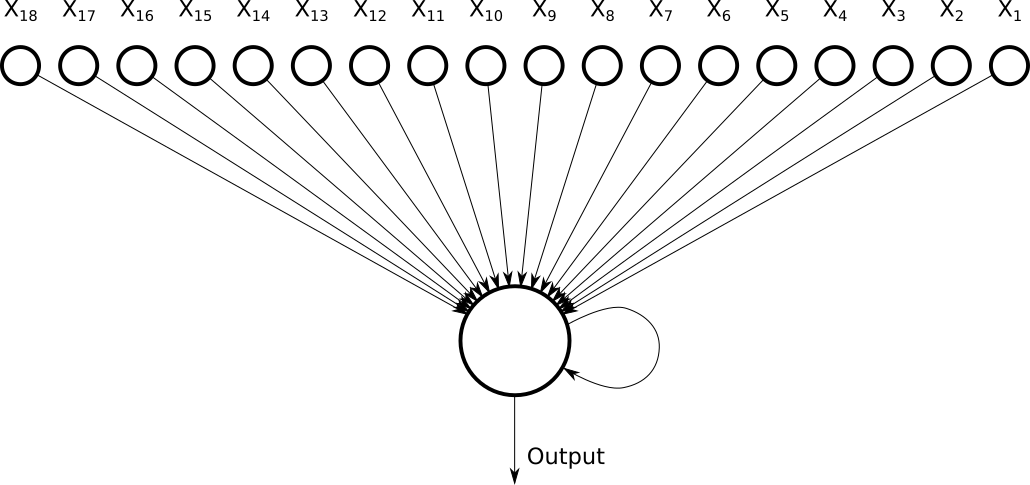
\includegraphics[width=1\linewidth]
    {gfx/rnn_1_topology}
  }
  \caption{First experiments \textit{RNN} topology.}
  \label{fig:rnn-1-topology}
\end{figure}

For the second and the third experiment, the features used are those
selected by \textit{WFSS}, which are \textit{total bitcoins} and
\textit{market price}. The second experiments layout which is shown in
\autoref{fig:rnn-8-topology} has as input layer two neurons for each
timestep. In the second layer, the first hidden layer, there are eight
\textit{RNN} neurons, one per timestep. Each one of those \textit{RNN}
neurons represent a timestep and is fed with the two corresponding
inputs and the previous timestep, which is the previous \textit{RNN}
neuron. After the \textit{RNN} hidden layer, there is an \textit{ANN}
hidden layer, with four neurons, fed by each one of the eight
\textit{RNN} neurons. Finally there is a single \textit{ANN} which
gives the output.

\begin{figure}[bth]
  \myfloatalign
  {
    \includegraphics[width=1\linewidth]
    {gfx/rnn_8_topology}}
  \caption{Second experiment \textit{RNN} topology.}
  \label{fig:rnn-8-topology}
\end{figure}

Just as in the second experiment, in the third we have four layers in
total, with one for the input, another one for the output and two
hidden layers. They are distributed similarly as those of the second
experiment. In the first layer there are two neurons for each
timestep, but in this third experiment we have 20 \textit{RNN}
neurons, fed by the two corresponding input neurons and the previous
timestep. After the \textit{RNN} hidden layer comes another
\textit{ANN} layer with 10 \textit{fully connected} neurons. Each one
of the \textit{ANN} neurons are fed by all the \textit{RNN} neurons of
the previous layer. Finally there is the output \textit{ANN} neuron.
The layout can be seen in \autoref{fig:rnn-20-topology}.

\begin{figure}[bth]
  \myfloatalign
  {
    \includegraphics[width=1\linewidth]
    {gfx/rnn_20_topology}}
  \caption{Third experiment \textit{RNN} topology.}
  \label{fig:rnn-20-topology}
\end{figure}

After the pre-processing, and to avoid over-fitting we have used
\textit{time series cross-validation} proposed by
\cite{robjhyndman2010}. The particular implementation of this
technique used uses a test partition of size 1, which we call $x_{t +
1}$ and a train partition composed of all the elements from the
$1095$-th to the $t$-th. The details about why we used $1095$-th as
the first element and the overall technique can be found in
\autoref{part:implementation}.

Regarding \textit{vector autoregression (VAR)} we had to choose two
parameters to build the model, one is the number of variables or
features and the other is the lags of each variable. For the features
used, as mentioned in \autoref{ch:feature-selection}, we used a
\textit{principal component analysis (PCA)} to select a subset of 18
features out of the original 41. After that, using \textit{wrapper
  feature subset selection (WFSS)} we chose a subset of those 18
features previously selected. The size and the particular features
selected in the last subset depends on the model used and the
parameters chosen. Considering this, we will explain first how did we
choose the lag parameter and then how that choice affected
\textit{WFSS} and the result of these process.

To set the lag parameter we have built an automated system to choose
from several information criteria available in the \textbf{vars}
package. This information criteria are, \textit{Akaike's information
  criteria (AIC)} by \cite{akaike1974new}, \textit{bayesian
  information criteria (BIC)} by \cite{schwarz1978estimating},
\textit{final prediction error (FPE)} by \cite{akaike1973infor} and
\textit{Hannan–Quinn information criterion (HQC)} by
\cite{hannan1979determination}. Once we have the lag parameter chosen
by the aforementioned information criteria, we order in ascending
order the set of lags obtained and select the first one, then perform
a \textit{Portmanteau's} test to check that the residuals are
uncorrelated. If the null hypothesis of \textit{no serial correlation}
is rejected we choose the next lag obtained. This process continues
until the null hypothesis is not rejected.

Once we have the lag parameter we perform a \textit{WFSS} to obtain a
feature subset. In the specific case of \textit{VAR}, the \textit{FSS}
obtained comprises the variables \textit{market price, Euro price in
  USD, cost per transaction percent, S\&P 500 volume, estimated
  transaction volume and S\&P 500 close}.

In the case of \textit{RNN}, there are multiple parameters to choose,
one of theme is the number of \textit{epochs}. Each \textit{epoch} is
a single pass on the entire data set to update the weights of the
network. In \textit{neural networks} the training process can be
stopped when the solution (weights and biases) has converged or after
a certain number of \textit{epochs}. In our case we chose to stop when
the solution has converged. But due to the computational cost of each
experiment, for the \textit{WFSS} phase we chose a fixed amount of 10
\textit{epochs}, which distorted the results, as the parameters for
\textit{WFSS} are different from the parameters used in the final
model building. This was done this way because we estimated the time
it would took to run all the \textit{WFSS} experiments in a single
computer would be 72 days, which is beyond the scope of this project.
Although the results has been distorted, they are good enough to take
them into the study as good approximations.

Another parameters are the number of \textit{hidden layers} and the
number of neurons in each \textit{hidden layer}. There isn't a
heuristic to choose the number of layers and neurons, and the more
layers and neurons you have, the more computational power you need to
learn the network parameters. As we shown before, we have chosen to
experiment with three different layouts to see how they compare and
observe how the changes in the model accuracy with the change of
certain parameters.

Learning rate is another parameter that controls the size of weight
and bias changes in learning of the training algorithm. \textit{Keras}
framework lets us add a regularization term to the cost function in
order to control the learning rate, we have added an \textit{L2} or
\textit{least square error} with parameter 0.001.

% If needed, the explanation behind regularization term is here:
% http://neuralnetworksanddeeplearning.com/chap3.html#overfitting_and_regularization

For the feature selection we also used the 18 features obtained with
\textit{PCA} and \textit{WFSS} for getting an even smaller feature
subset. In this case the subset was computed, as mentioned before, by
using a number of \textit{epochs} equal to 10, in order to run the
experiment in a reasonable amount of time. The subset obtained is
comprised of two variables, namely \textit{market price} and
\textit{total Bitcoins}.

\chapter{Experimental Results}
\label{ch:experimental-results}

\section{Results introduction}
\label{sec:result-presentation}

% TODO: Here we are

In this section we present the results for four experiments to compare
the performance of two different models \textit{recurrent neural
  network (RNN)} and \textit{vector autoregression (VAR)}, being
\textit{RNN} configured in three different ways. The first
\textit{RNN} configuration, previously introduced in
\autoref{ch:experimental-setup}, called simply \textbf{RNN}, is a
\textit{RNN} with the 18 features selected by \textit{PCA} as input
which feed one single \textit{recurrent neuron}. The second is an
\textit{RNN} with 8 \textit{recurrent neurons} and uses only the two
features selected by \textit{WFSS} as input, this configuration is
called \textbf{RNN 8}. The third configuration used is called
\textbf{RNN 20}, with 20 \textit{recurrent neurons} and also uses the
two features selected by \textit{WFSS}.

Both \autoref{fig:predictions-subplots} and \autoref{fig:predictions}
represent a day ahead prediction of the Bitcoin price, compared to the
real Bitcoin price, shown in the variable \textit{MarketPrice}. It is
the same information presented in two different ways to allow the
viewer to see the particular values of each one in
\autoref{fig:predictions-subplots}, and, on the other side, to be able
to compare closely the values of the two models and
\textit{MarketPrice} in \autoref{fig:predictions}.

\begin{figure}[bth]
  \myfloatalign {
    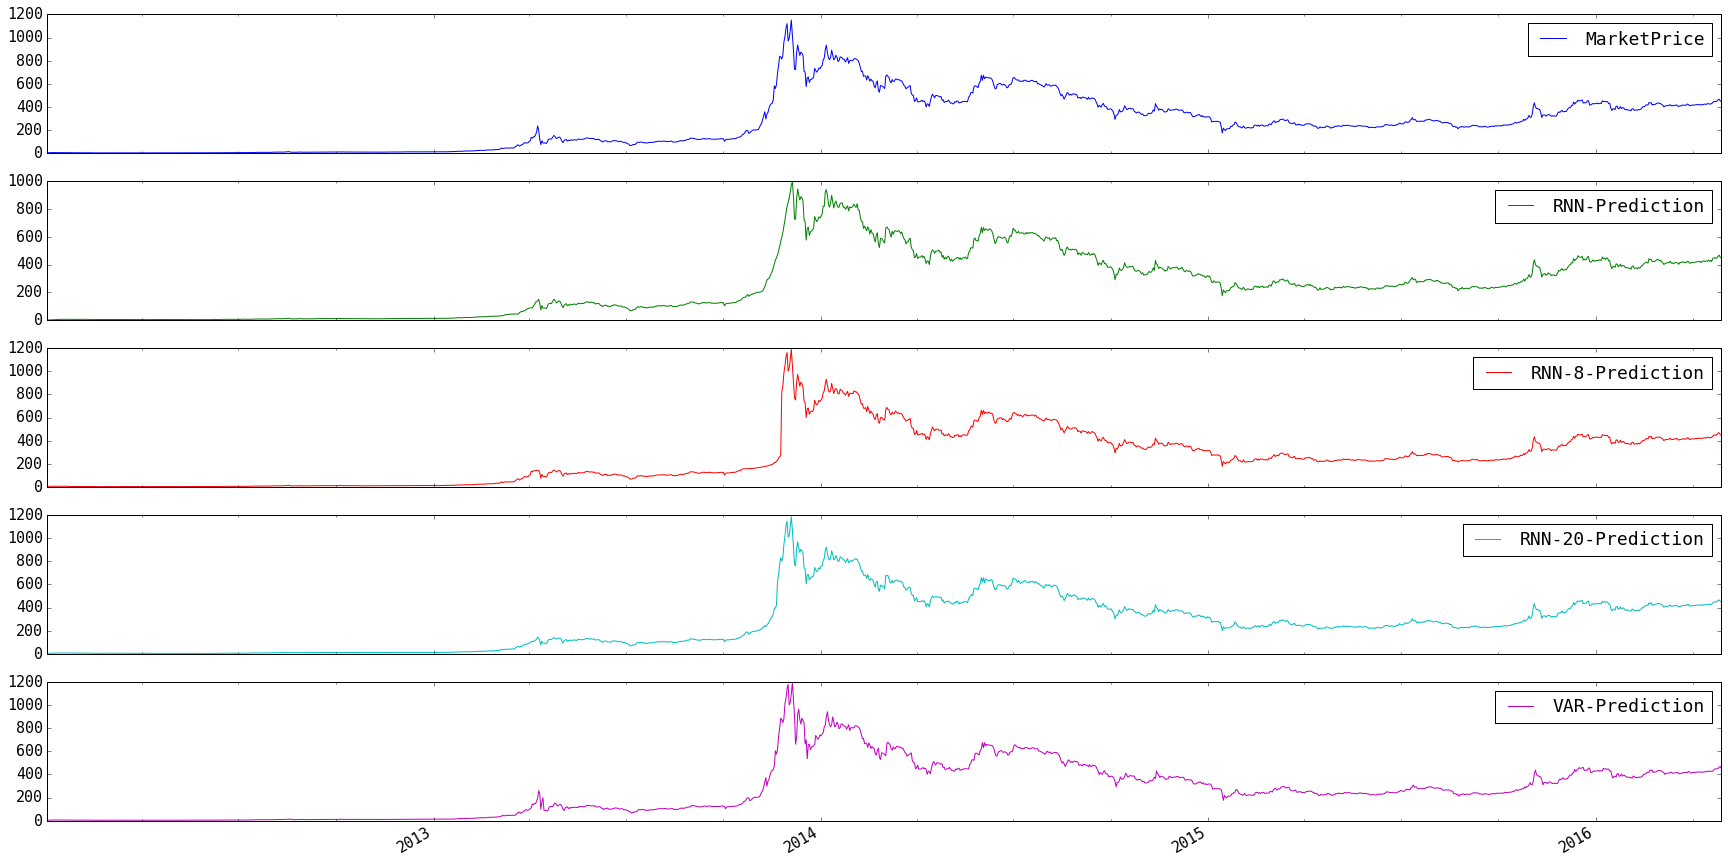
\includegraphics[width=1\linewidth]
    {gfx/prediction-subplots}}
  \caption{Prediction models and \textit{MarketPrice} true values in
    separate charts.}
  \label{fig:predictions-subplots}
\end{figure}

Although the shapes of the charts are similar, it can be noticed how
\textit{RNN} takes more instances to learn certain patterns. We can
see that \textbf{RNN} performs better than \textbf{RNN 8}. In this
particular case, more features help to learn more rapidly from the
data. But when we increase the number of \textit{recurrent input
  neurons}, which is the same as saying that we increase the window of
the input time series, we get better results without resorting to the
use of more features. There is a comparison of forecast accuracy
measures that reflect the intuitions observed before in
\autoref{tab:forecast-accuracy-measures}.

\textit{RNN}, with the exception of \textbf{RNN 20}, has a tendency to
predict lower values than those predicted by \textit{VAR} and
\textit{MarketPrice}. When the change in the price is high
\textit{RNN} doesn't change at the same pace while \textit{VAR}
follows the tendency better. This behavior is better perceived in the
upper-right and lower-left chart of \autoref{fig:predictions}.

\begin{figure}[bth]
  \myfloatalign {
    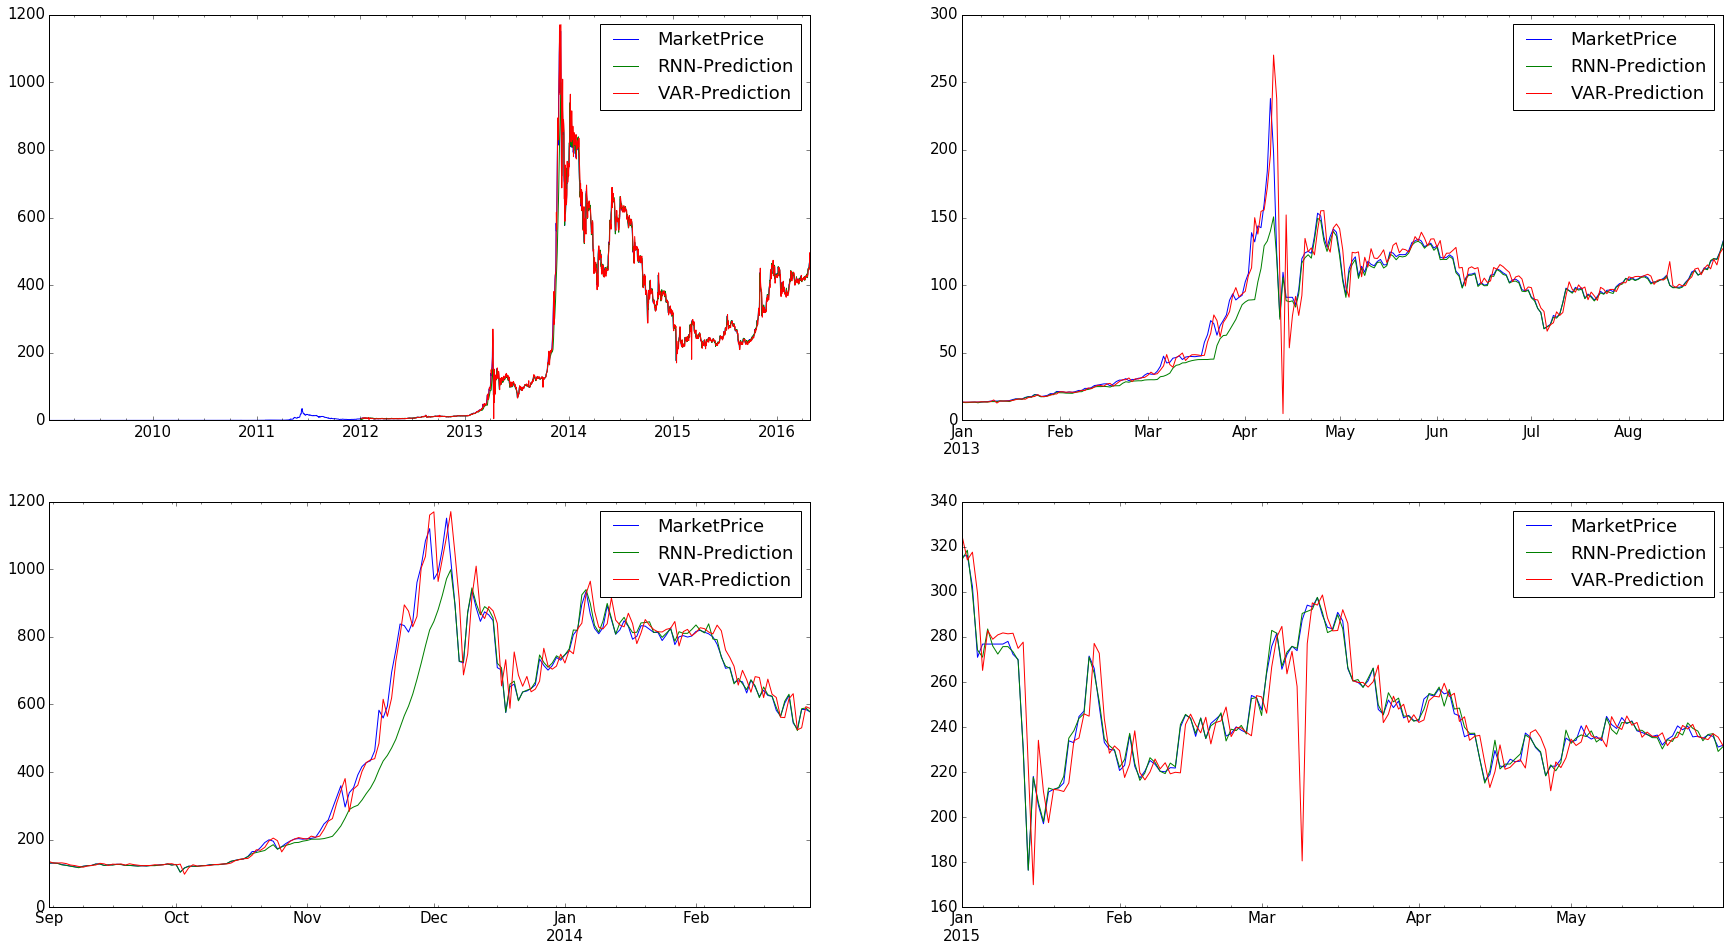
\includegraphics[width=1\linewidth]
    {gfx/predictions}}
  \caption{Prediction models and \textit{MarketPrice} true values in
    the same chart.}
  \label{fig:predictions}
\end{figure}

\section{Accuracy measures}
\label{sec:accuracy-measures}

\begin{table}[bth]
  \myfloatalign
  \tiny
  \begin{tabularx}{\textwidth}{Xcccc}
    \toprule \tableheadline{Measure Type}
    & \tableheadline{RNN Value}
    & \tableheadline{RNN 8 WFSS Value}
    & \tableheadline{RNN 20 WFSS Value}
    & \tableheadline{VAR Value} \\
    \midrule
    \textit{Mean absolute error (MAE)} & $5.4$ & $6.53$ & $4.51$ &  $7.62$ \\
    \textit{Mean squared error (MSE)} & $638.55$ & $1282.43$ & $189.5$ & $325.60$ \\
    \textit{Mean absolute percentage error (MAPE)} & $3.19$ & $2.39$ & $3.7$ & $2.79$ \\
    \textit{Theil's U statistic} & $0.47$ & $0.08$ & $0.01$ & $0.03$ \\
    \bottomrule
  \end{tabularx}
  \caption{Forecast accuracy measures}
  \label{tab:forecast-accuracy-measures}
\end{table}

The main accuracy measure used is \textit{mean absolute error (MAE)},
shown in \autoref{eq:mae-expression}. \textit{MAE} averages the
absolute error produced for every prediction done with a particular
model. This error measure has the characteristic of representing
quantities in the same unit as the original variable and that is
easily understandable.

When the fluctuation of the \textit{BTC} price are low, \textit{RNN}
is closer to \textit{MarketPrice} than \textit{VAR}, which can be seen
in \autoref{fig:comparison-histogram-prediction-errors}.

\begin{equation}
  \begin{aligned}
    \label{eq:mae-expression}
    \textit{Mean Absolute Error: MAE} & =
    \frac{1}{n} \sum_{i=1}^{n} |y_i - \hat{y}_i|.\\
  \end{aligned}
\end{equation}

The next accuracy measure is \textit{mean squared error (MSE)}, shown
in \autoref{eq:mse-expression}, which doesn't present the prediction
errors in the same unit, but has the feature of giving more importance
to bigger errors than smaller ones. To see how this two measures gives
us different information about the same data we can see in
\autoref{tab:forecast-accuracy-measures} that, while \textit{RNN}'s
\textit{MAE} is lower than \textit{VAR}'s \textit{MAE}, the
\textit{RNN}'s \textit{MSE} for \textbf{RNN} and \textbf{RNN 8} is
bigger than \textit{VAR}'s. That is because for \textbf{RNN} and
\textbf{RNN 8} big errors are bigger and at the same time it has less
small errors. That can be clearly seen in
\autoref{fig:comparison-histogram-prediction-errors}.

\begin{figure}[bth]
  \myfloatalign {
    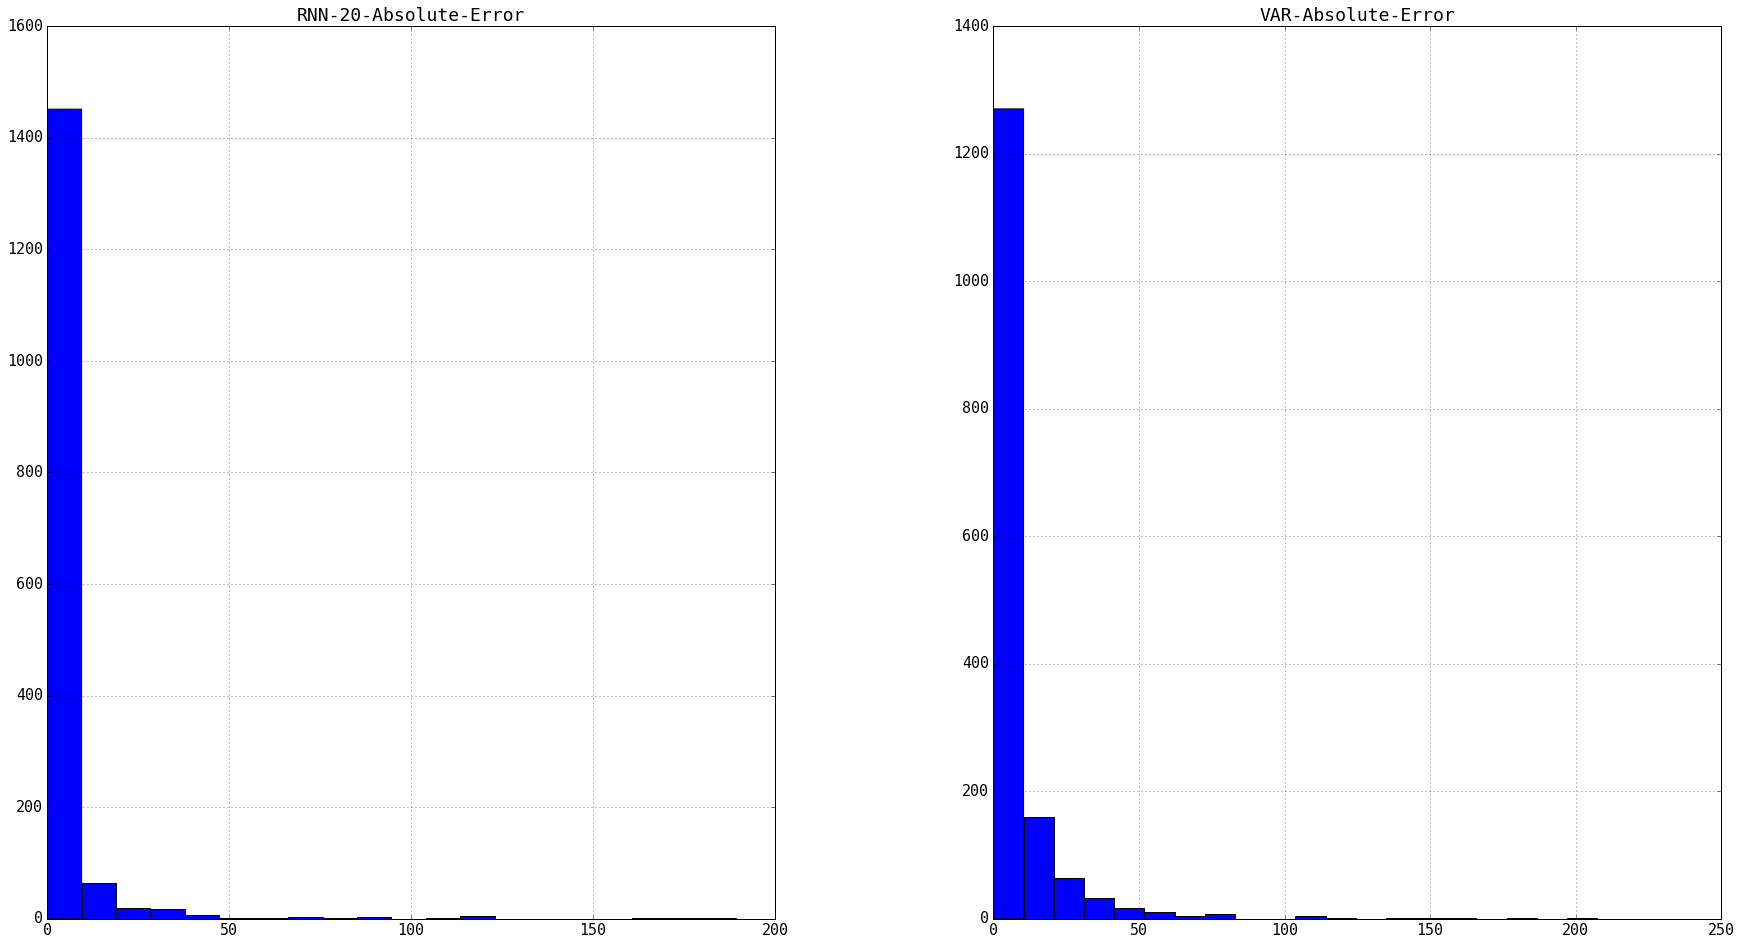
\includegraphics[width=1\linewidth]
    {gfx/comparison-histogram-prediction-errors}}
  \caption{Histogram of \textit{RNN} absolute errors and \textit{VAR}
    absolute errors.}
  \label{fig:comparison-histogram-prediction-errors}
\end{figure}

\begin{equation}
  \begin{aligned}
    \label{eq:mse-expression}
    \textit{Mean Squared Error: MSE} & = \frac{1}{n} \sum_{i=1}^{n}
    (y_i - \hat{y}_i)^2.\\
  \end{aligned}
\end{equation}

Another accuracy measure used is \textit{mean absolute percentage
error (MAPE)}, defined in \autoref{eq:mape-expression}. This measure
is useful when there are several scales, for example if the models are
run over different data-sets. This measure have the disadvantage of
being undefined for $y_i = 0$, and that it puts a heavier penalty on
negative errors than on positive errors.

\begin{equation}
  \begin{aligned}
    \label{eq:mape-expression}
    \textit{Mean Absolute Percentage Error: MAPE} & = \frac{100}{n}
    \sum_{i=1}^{n} \frac{y_i - \hat{y}_i}{y_i}.
  \end{aligned}
\end{equation}

Finally we include \textit{Theil's U statistic} which is defined in
\autoref{eq:theils-u-statistic}. This measure compares a forecast
model to the actual model. Is the ratio of the 1-step-ahead
\textit{MSE} for a given forecast relative to that of a random walk
forecast. If \textit{Theil's U statistic} is less than 1 then the
forecasting technique is better than guessing, if is exactly 1 then is
about as good as guessing and if it is more than 1 the forecasting
technique is worse than guessing.

\begin{equation}
  \begin{aligned}
    \label{eq:theils-u-statistic}
    \textit{Theil's U statistic} & = \sqrt{\frac {\displaystyle\sum_{t
          = 1}^{n - 1} \left( \frac{\hat{y}_{t+1} - y_{t+1}}{y_t}
        \right)^2} {\displaystyle\sum_{t = 1}^{n - 1} \left(
          \frac{y_{t+1} - y_t}{y_t} \right)^2}}.
  \end{aligned}
\end{equation}

We can see in \autoref{tab:forecast-accuracy-measures} that the value
of \textit{Theil's U statistic} for all the models is less than one,
hence we can assume that this models are better forecasting techniques
than guessing.

\textbf{RNN 8} is the closest to one followed by \textbf{RNN}, then
\textbf{VAR} and finally \textbf{RNN 20}. We can observe here, as well
as in the charts and previous forecasting accuracy measures, that the
number of features selected and the number of \textit{recurrent input
neurons} are two parameters that have a big impact on the performance
of the \textit{RNN} model.

\section{Errors analysis}
\label{sec:errors-analysis}

\autoref{fig:comparison-errors} shows an important information to be
able to understand how do the two prediction models studied behave.

\begin{figure}[bth]
  \myfloatalign
  {
    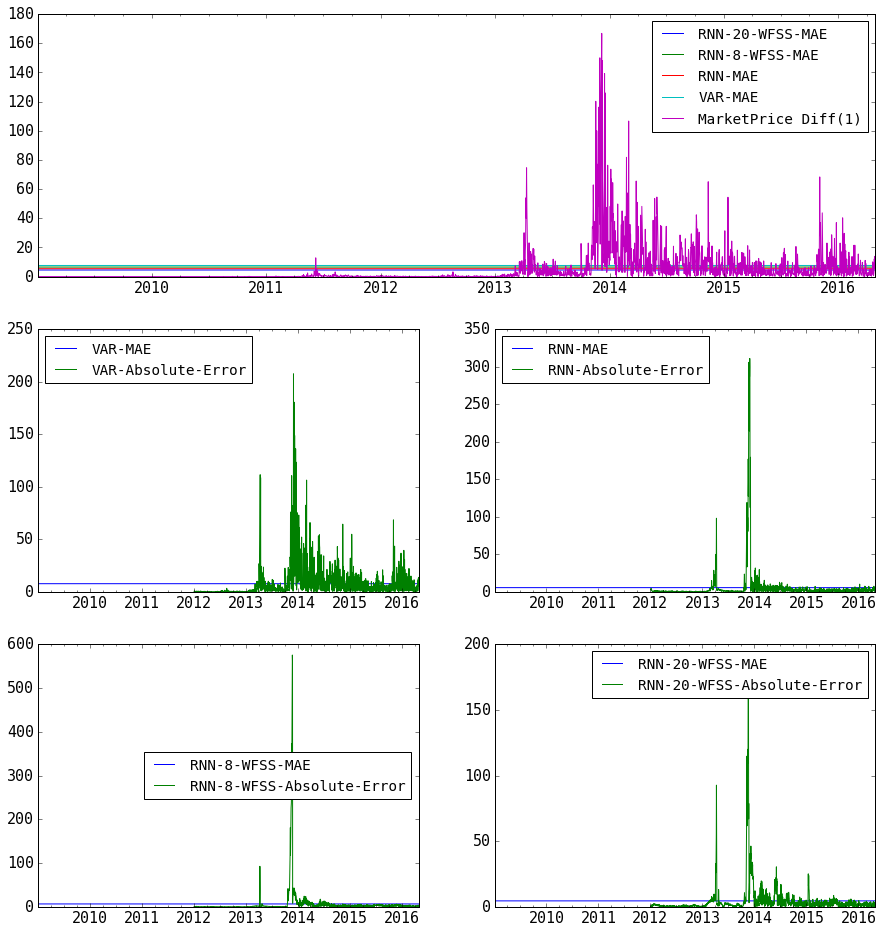
\includegraphics[width=1\linewidth]
    {gfx/comparison-errors}}
  \caption{Error graphs.}
  \label{fig:comparison-errors}
\end{figure}

First off we can see the comparison between the \textit{MAE}'s of each
model and the fluctuation (formally know as first difference or
\textit{Diff(1)}) of the \textit{BTC} price. It's important to note
that for the two models the \textit{MAE} is mostly beneath the daily
fluctuation of \textit{BTC}, which tells us the the error is
relatively small to predict the \textit{MarketPrice}.

In the two lower graphs of \autoref{fig:comparison-errors} we see a
comparison of model's \textit{MAE} and absolute errors. The errors of
\textit{RNN} are located around two events of huge change of the
\textit{MarketPrice}. There the errors of \textbf{RNN 20} are lower
than those of \textit{VAR}, but those of \textbf{RNN} and \textbf{RNN
  8} are larger. That's the reason why \textbf{RNN} and \textbf{RNN 8}
have larger \textit{MSE} than \textit{VAR}, while \textbf{RNN 20} has
lower \textit{MSE} than \textit{VAR}, because bigger errors are
penalized. Besides, in the rest of the time series the errors of
\textit{VAR} exceed those of \textit{RNN}, which is the reason why
\textit{RNN's} \textit{MAE} is lower than \textit{VAR's}.

Regarding the errors probability distribution we would benefit from it
to be normal, because that way we would be able to establish a
confidence interval with the normal distribution parameters with the
expression in \autoref{eq:confidence-interval}.

\begin{equation}
  \begin{aligned}
    \label{eq:confidence-interval}
    \textit{Confidence interval} & =
    [ \hat{x} - 2 \sigma, \hat{x} + 2 \sigma ].
  \end{aligned}
\end{equation}

In \autoref{fig:normal-fitted-to-errors} we can see the shape of the
error's histograms plotted along a fitted normal distribution.
Visually the shape of the normalized histograms resembles that of the
fitted normal distributions but we need more evidence. Hence we've run
several normality tests in order to ensure that the distribution of
the errors can be considered to be normal.

\begin{figure}[bth]
  \myfloatalign
  {
    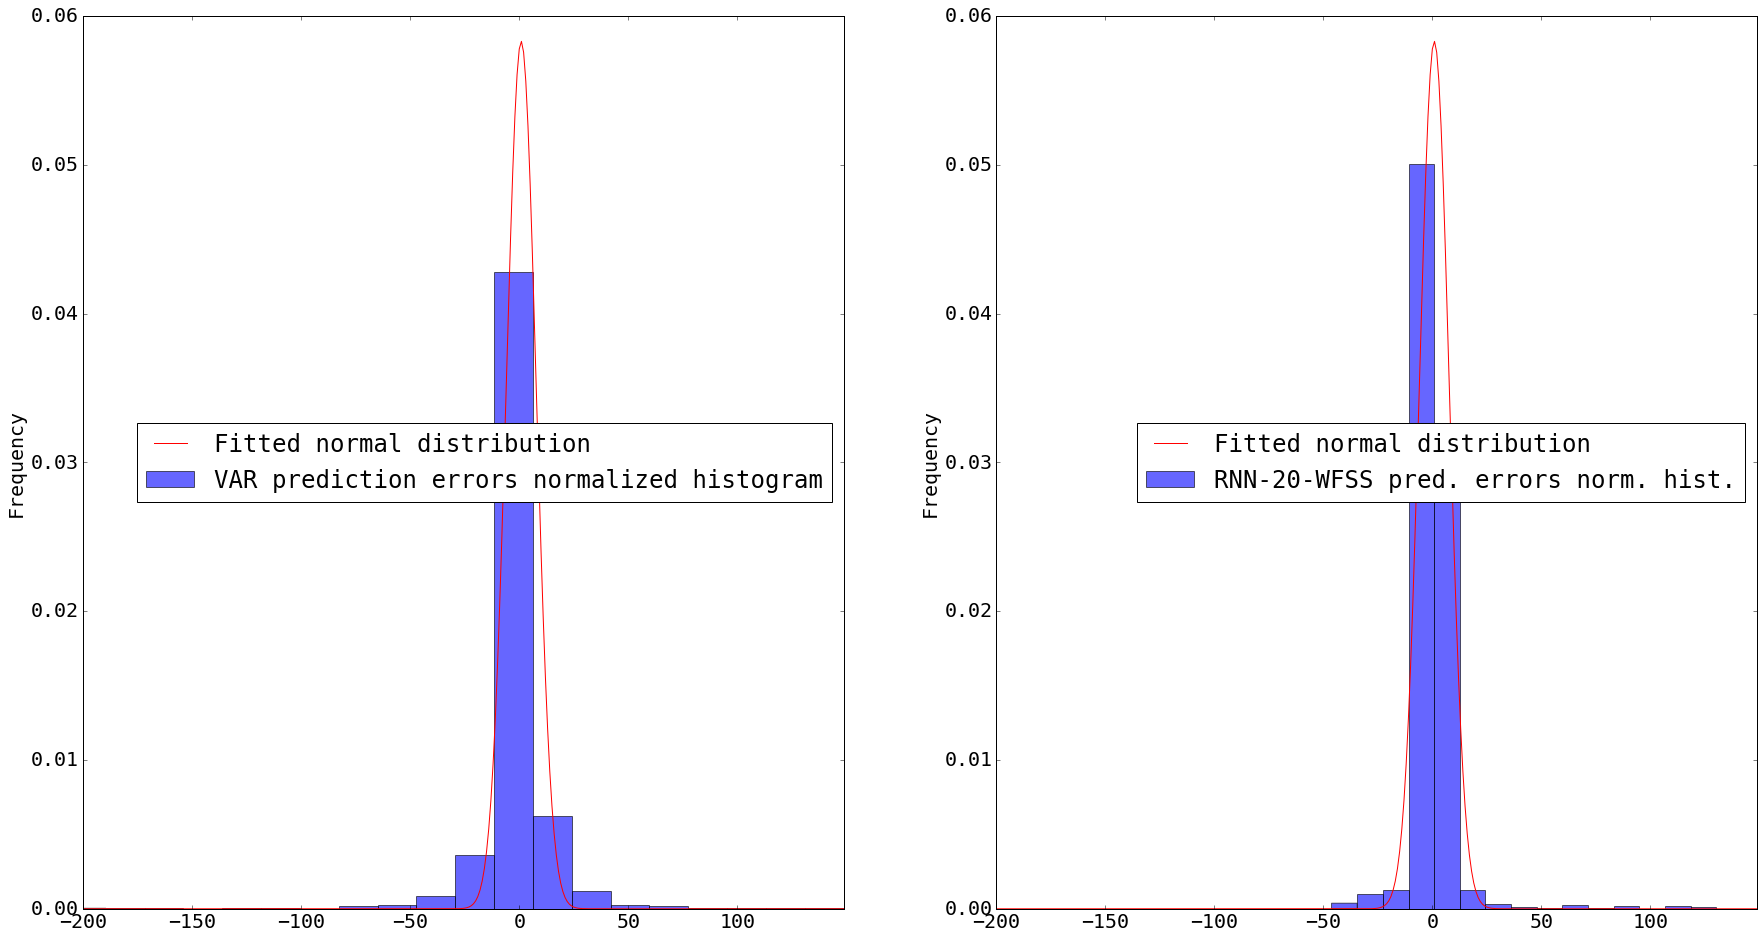
\includegraphics[width=1\linewidth]
    {gfx/normal-fitted-to-errors}}
  \caption{Normal fitted to prediction errors.}
  \label{fig:normal-fitted-to-errors}
\end{figure}

In \autoref{tab:normality-test-results} we can see the results of all
the normality tests performed, namely \textit{skewness test},
\textit{kurtosis test}, and \textit{D’Agostino and Pearson's
``omnibus'' test}.

\textbf{Skewness} (\cite{d1970transformation}) - Is a measure of the
asymmetry of the probability distribution of a random variable about
it's mean. In other words, skewness tells you the amount and direction
of skew (departure from horizontal symmetry). The skewness value can
be positive or negative, or even undefined. If skewness is $0$, the
data are perfectly symmetrical, although it is quite unlikely for
real-world data. As a general rule of thumb:

\begin{itemize}
\item If skewness is less than -1 or greater than 1, the distribution
  is highly skewed.
\item  If skewness is between -1 and -0.5 or between 0.5
  and 1, the distribution is moderately skewed. 
\item If skewness is between
  -0.5 and 0.5, the distribution is approximately symmetric.
\end{itemize}

The mathematical expression of the skewness measure is defined in
\autoref{eq:skewness-measure}.

\begin{equation}
  \begin{aligned}
    \label{eq:skewness-measure}
    & \textit{Skewness Measure} = \frac{m_3}{m_2^{3/2}}, \textit{
      where } m_k = \frac{1}{n} \displaystyle\sum_{i=1}^n (e_i - \bar{e} )^k
  \end{aligned}
\end{equation}

\begin{table}[bth]
  \myfloatalign
  \tiny
  \begin{tabularx}{\textwidth}{Xcc}
    \toprule \tableheadline{Type of test} &
    \tableheadline{Statistic test value}
    & \tableheadline{P-Value} \\
    \midrule
    \textit{VAR Skewness test} & $-24.11$ & $1.69e-128$ \\
    \textit{RNN 20 WFSS Skewness test} & $38.29$ & $0.0$ \\
    \textit{VAR Kurtosis test} & $22.39$ & $4.57e-111$ \\
    \textit{RNN 20 WFSS Kurtosis test} & $24.55$ & $3.84e-133$ \\
    \textit{VAR D’Agostino and Pearson omnibus test} & $1083.04$ & $6.61e-236$ \\
    \textit{RNN 20 WFSS D’Agostino and Pearson omnibus test} & $2069.63$ & $0.0$ \\
    \bottomrule
  \end{tabularx}
  \caption{Normality test results}
  \label{tab:normality-test-results}
\end{table}

We can see by the results of the test in
\autoref{tab:normality-test-results} that the distribution of the
errors of the two models are skewed.

\textbf{Kurtosis} (\cite{anscombe1983distribution}) - This measure is
informative about the tail behavior of a series. \textit{Kurtosis}
tells the height and sharpness of the central peak, relative to that
of a standard bell curve. A distribution with positive
\textit{kurtosis} has heavier trails and a higher peak than the
normal, whereas a distribution with negative \textit{kurtosis} has
lighter trails and is flatter. Why are tailedness and peakedness both
components of \textit{kurtosis}? It is basically because
\textit{kurtosis} represents a movement of mass that does not affect
the variance. Consider the case of positive \textit{kurtosis}, where
heavier tails are often accompanied by a higher peak. Note that if
mass is simply moved from the shoulders of a distribution to it's
tails, then the variance will also be larger. To leave the variance
unchanged, one must also move mass from the shoulders to the center,
which gives a compensating decrease in the variance and a peak. For
negative \textit{kurtosis}, the variance will be unchanged if mass is
moved from the tails and center of the distribution to it's shoulders,
thus resulting in light tails and flatness. The mathematical
expression is shown in \autoref{eq:kurtosis-measure}.

\begin{equation}
  \begin{aligned}
    \label{eq:kurtosis-measure}
    \textit{Kurtosis Measure} = \frac{m_4}{m_2^2} - 3, \text{ where }
    m_k = \frac{1}{n} \displaystyle\sum_{i=1}^n (e_i - \bar{e})^k
  \end{aligned}
\end{equation}

\textbf{D’Agostino and Pearson omnibus} (\cite{d1971omnibus,
d1973tests}) - This test is a combination of \textit{skewness} and
\textit{kurtosis}, called \textit{``omnibus''} test. The mathematical
expression is \autoref{eq:omnibus-measure}. The distribution of the
\textit{``omnibus''} measure is approximately a $\chi^2$ distribution
with two degrees of freedom under the null hypothesis that the sample
was drawn from a population with normally distributed values.

\begin{equation}
  \begin{aligned}
    \label{eq:omnibus-measure}
    \textit{Omnibus Measure} =
    ((\frac{m_3}{m_2^{3/2}})^2 + (\frac{m_4}{m_2^2})^2, \text{ where }
    m_k = \frac{1}{n} \displaystyle\sum_{i=1}^n (e_i - \bar{e} )^k
  \end{aligned}
\end{equation}

Given that the null hypothesis is that the samples in the errors set
are drawn from a normal distribution and the p-values are less than
0.01, the aforementioned null hypothesis gets rejected. In light of
this results we can't conclude that the errors are normally
distributed.

\section{Results for 2013 onwards}
\label{sec:results-for-2013-onwards}

It's interesting to look at the results of the range of all
predictions made after 2013, there are barely fluctuations of the BTC
price.

Both \autoref{fig:prediction-range-2013-subplots} and
\autoref{fig:prediction-range-2013} are basically the same figures as
\autoref{fig:predictions-subplots} and \autoref{fig:predictions}
without the values before 2013.

\begin{figure}[bth]
  \myfloatalign {
    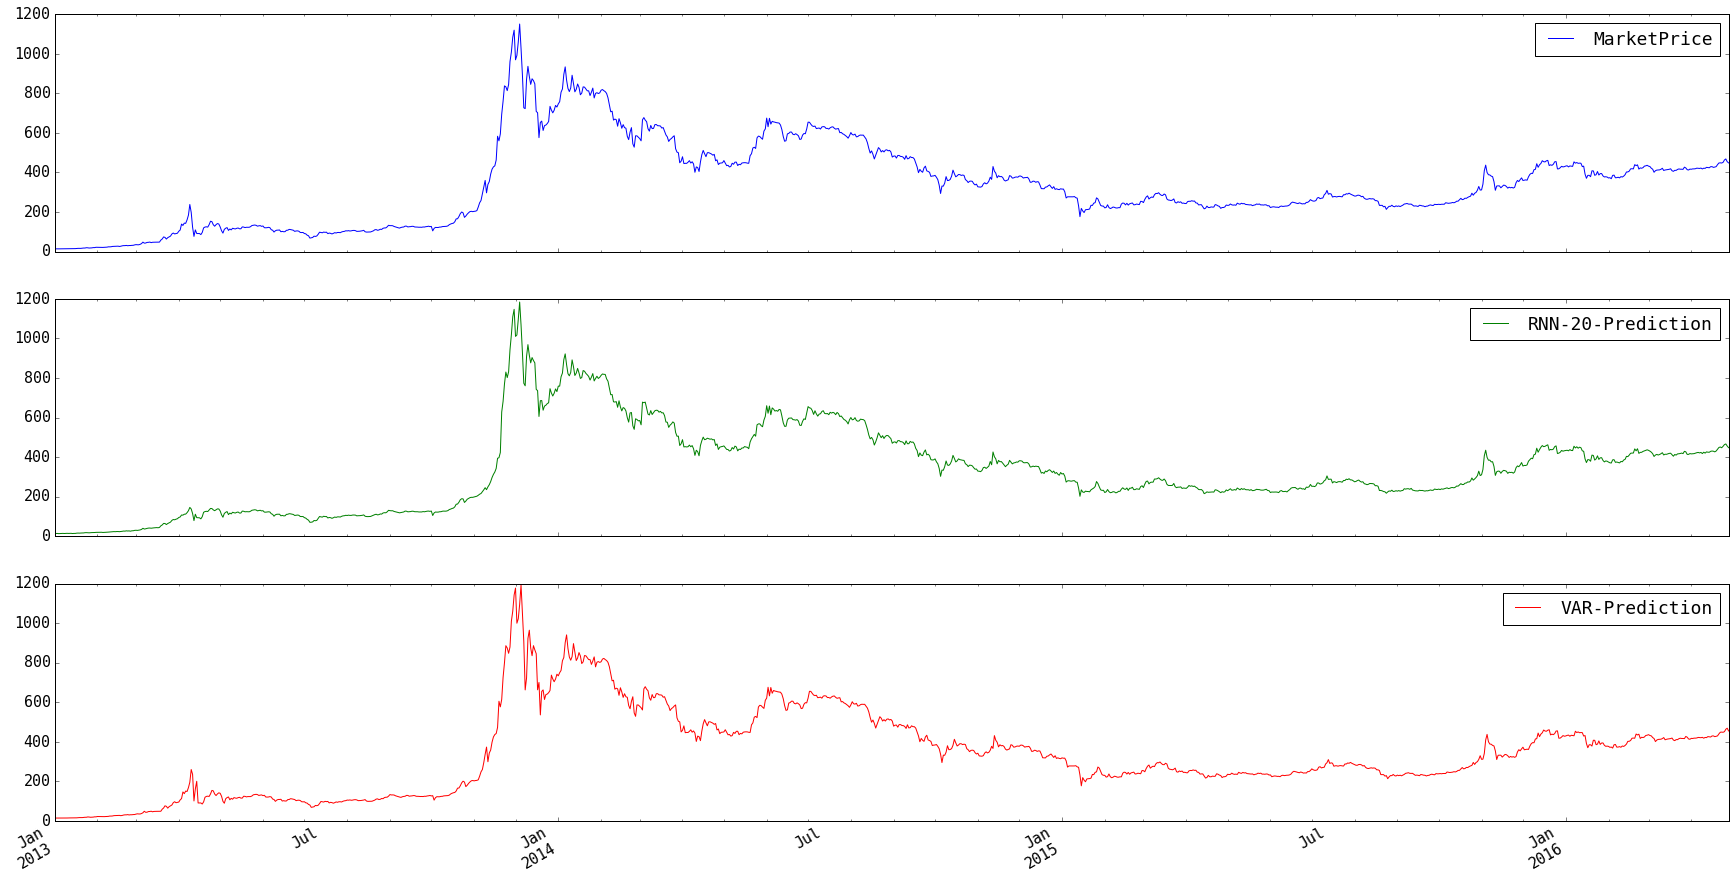
\includegraphics[width=1\linewidth]
    {gfx/prediction-range-2013-subplots}}
  \caption{Prediction models and \textit{MarketPrice} in separate
    plots for 2013 onwards.}
  \label{fig:prediction-range-2013-subplots}
\end{figure}

Because this range of the time series has more fluctuations, the
predictions have larger error measures than the predictions made with
the whole time series considered in \autoref{sec:result-presentation}.

\begin{figure}[bth]
  \myfloatalign {
    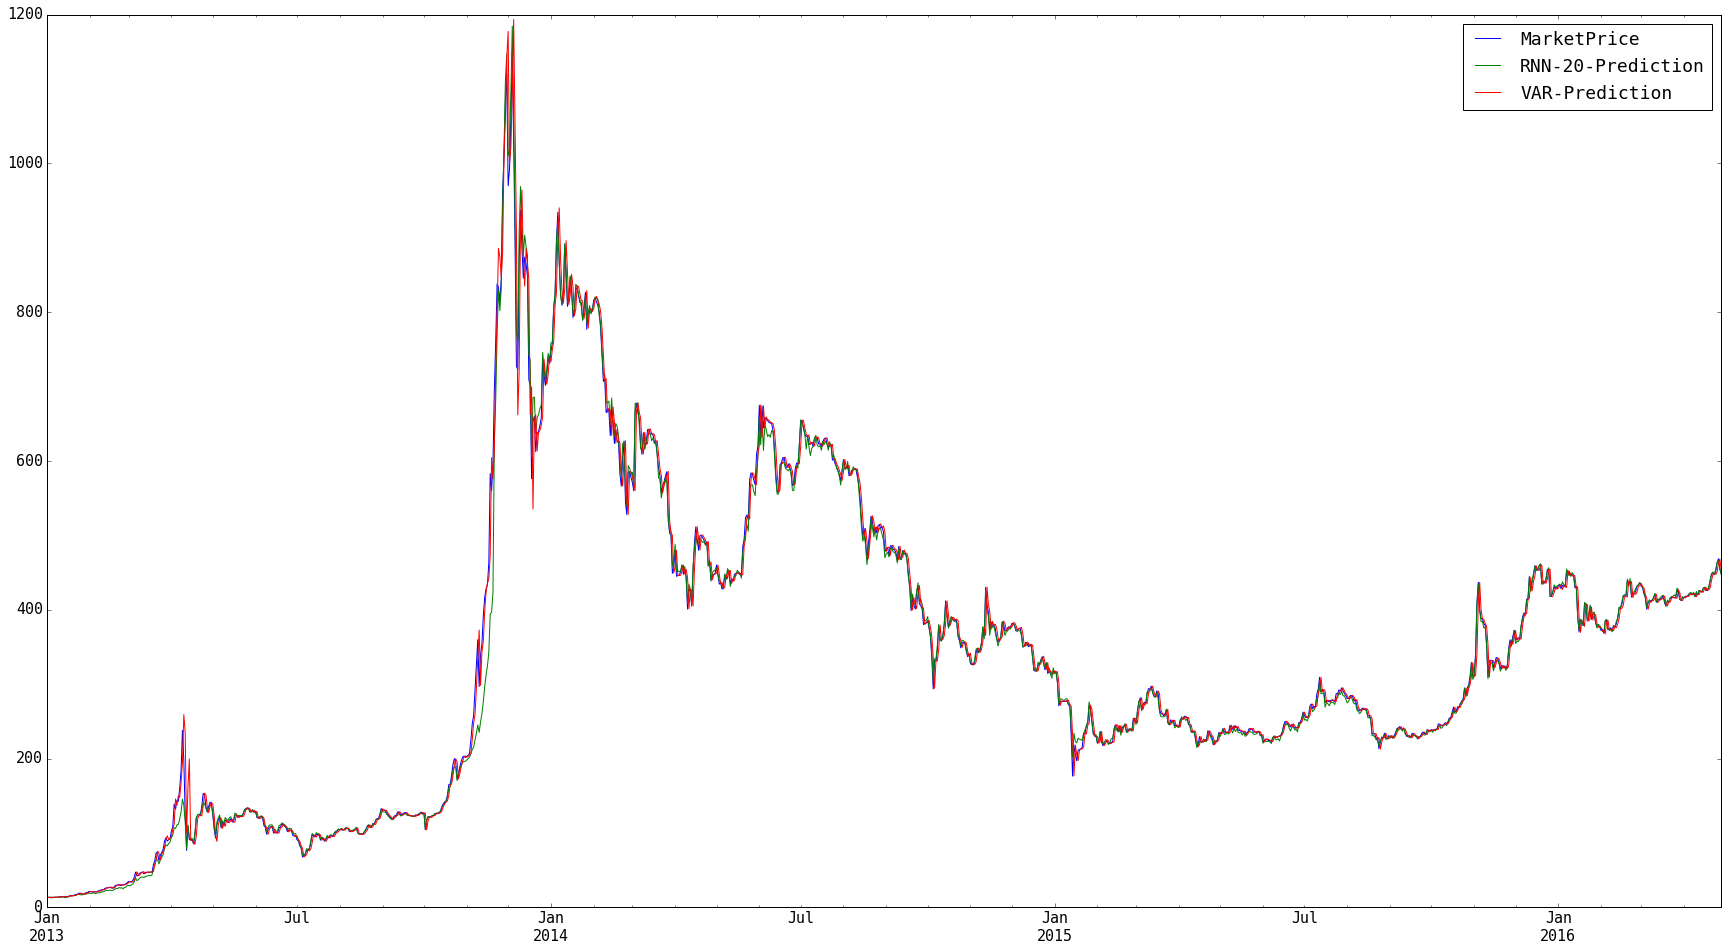
\includegraphics[width=1\linewidth]
    {gfx/prediction-range-2013}}
  \caption{Prediction models and \textit{MarketPrice} for 2013 onwards.}
  \label{fig:prediction-range-2013}
\end{figure}

In \autoref{tab:forecast-accuracy-measures-2013-onwards} it can be
seen how the error measures have increased and how the \textit{Theil's
U statistic} has decreased, been farther from 1, which means that
\textit{RNN} and \textit{VAR} are better predictors for the current
range than for the original range in
\autoref{tab:forecast-accuracy-measures-2013-onwards}.

\begin{table}[bth]
  \myfloatalign
  \tiny
  \begin{tabularx}{\textwidth}{Xcc}
    \toprule \tableheadline{Measure Type} &
    \tableheadline{RNN 20 WFSS Value}
    & \tableheadline{VAR Value} \\
    \midrule
    \textit{Mean absolute error (MAE)} & $5.67$ & $9.85$ \\
    \textit{Mean squared error (MSE)} & $246.13$ & $423.19$ \\
    \textit{Mean absolute percentage error (MAPE)} & $2.22$ & $3.04$ \\
    \textit{Theil's U statistic} & $0.01534$ & $0.03588$ \\
    \bottomrule
  \end{tabularx}
  \caption{Forecast accuracy measures for 2013 onwards}
  \label{tab:forecast-accuracy-measures-2013-onwards}
\end{table}

%---------------------------------------------------------------------
%---------------------------------------------------------------------
%---------------------------------------------------------------------

%\enlargethispage{2cm}

%------------------------------------------------

%%% Local Variables:
%%% mode: latex
%%% TeX-master: "../main"
%%% End:
